% Appendices
% To be used with hyper links

\begin{frame}[label=Convolutional_Layers]
  \frametitle{\acl{CNN}: Convolutional Layers}

  \begin{textblock}{90}(5, 10)
    \begin{center}
      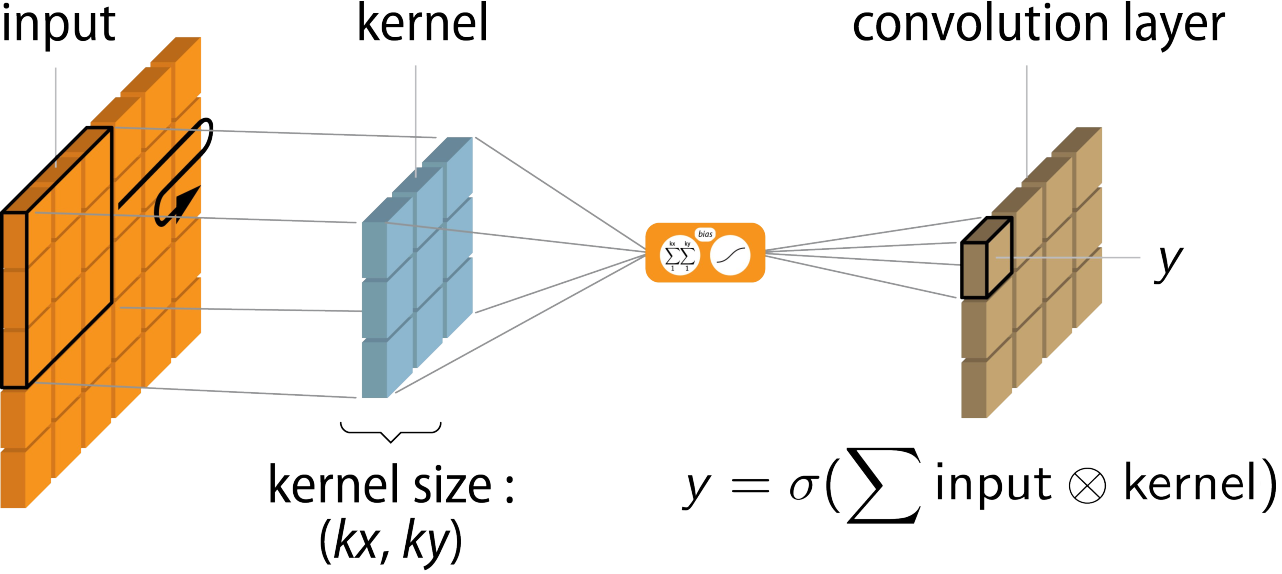
\includegraphics[width=\textwidth]{img/Convolution.png}
      Taken from FIDLE
    \end{center}
  \end{textblock}

  % Cheat a bit on the size
  \begin{textblock}{46}(5, 75)
    \begin{itemize}
    \item Common operation in image processing
    \item $\matrix{K}$ acts as a filter
    \end{itemize}
    \hyperlink{CNN_Overview_Convolutional}{\beamergotobutton{Go back}}
  \end{textblock}

  \begin{textblock}{45}(50, 75)
    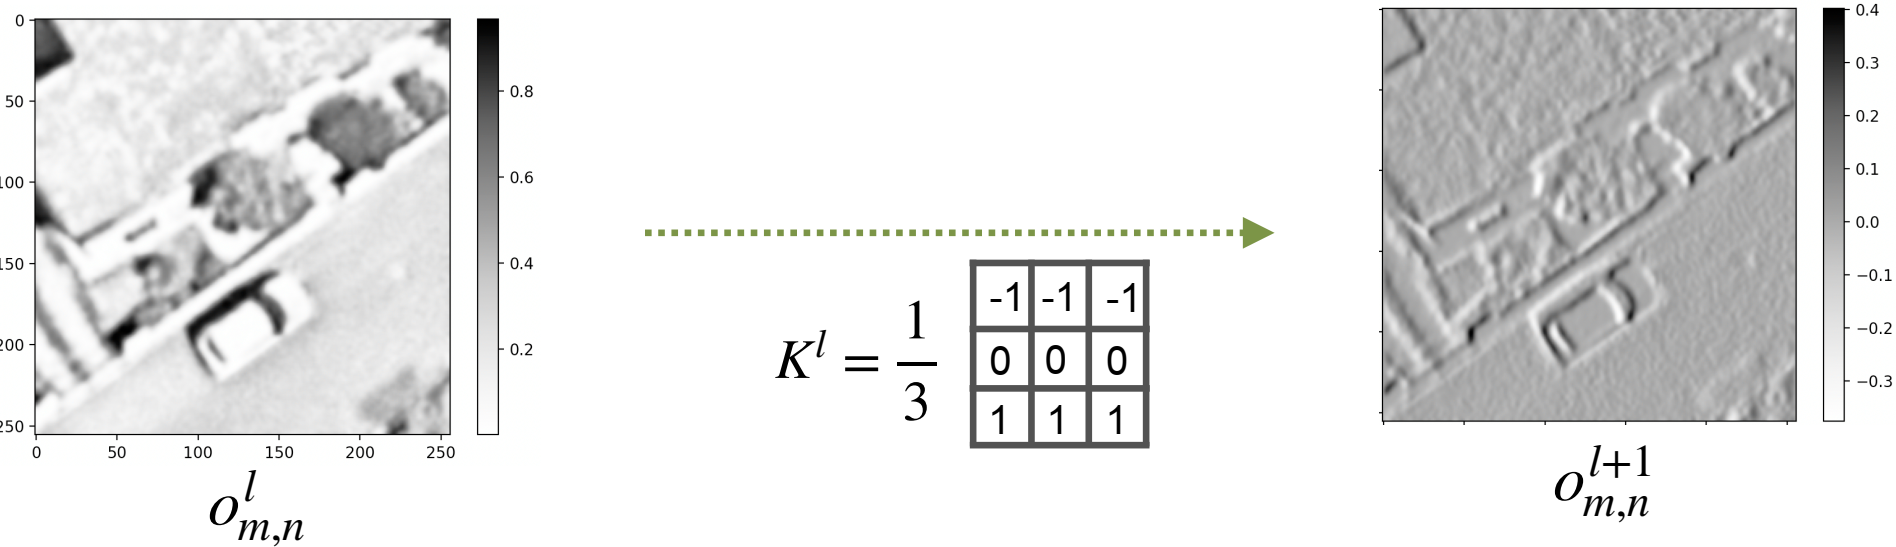
\includegraphics[width=\textwidth]{img/CNN_Filter.png}
  \end{textblock}
\end{frame}


\begin{frame}[label=Pooling_Layers]
  \frametitle{\acl{CNN}: Pooling Layers}

  \begin{textblock}{90}(5, 10)
    \begin{center}
      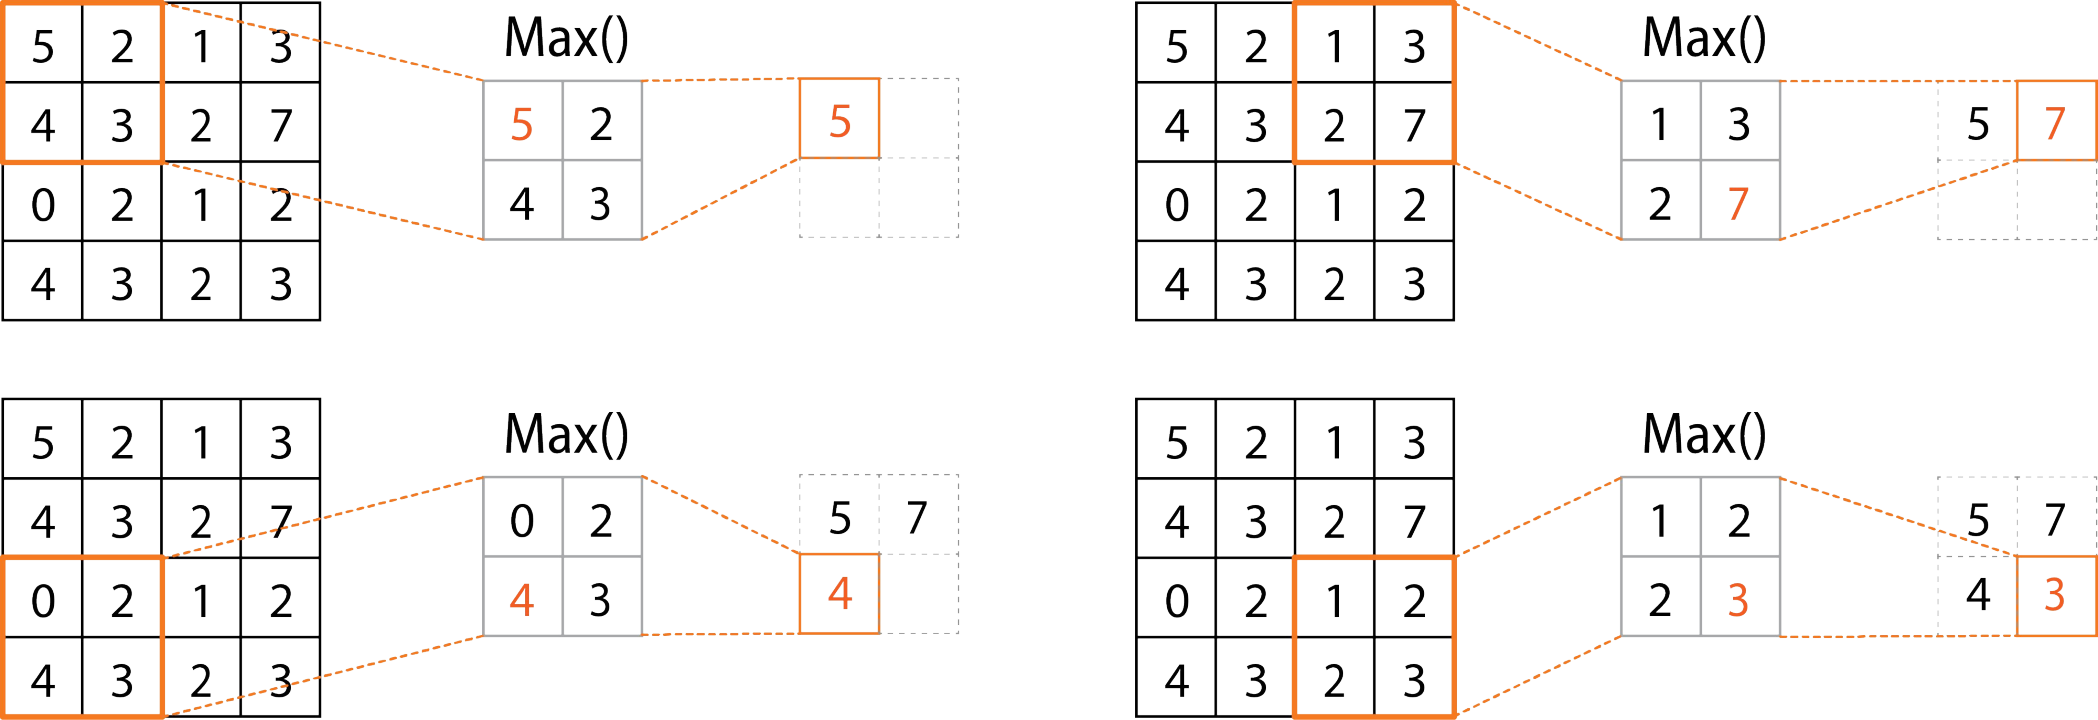
\includegraphics[width=\textwidth]{img/CNN_Pooling.png}
      Taken from FIDLE
    \end{center}
  \end{textblock}

  \begin{textblock}{90}(5, 75)
    Crude downsampling (dimensionality reduction)\\
    \hyperlink{CNN_Overview_Pooling}{\beamergotobutton{Go back}}
  \end{textblock}
\end{frame}
